\documentclass[MTRX3700report.tex]{subfiles}
% Lydia
%\documentclass{article}
%\usepackage{graphicx}
%\usepackage{float}
%\usepackage{listings}

\begin{document}
	
	\subsection{Module Requirements: Manual Mode}
	
	The Manual Mode module consists of all the control for the robot during manual mode. This module takes the user inputs from the controller to:
	
	\begin{enumerate}
		\item \textbf{Start and Stop} the movement of the robot immediately when the controller commands.
		\item \textbf{Control the Movement} of the robot through the joystick values sent from the controller. Moves forward, back, turns left and turns right.
		\item \textbf{Control the Speed} of the robot through the Global variable MAX\textunderscore SPEED set by the user through controller.
		\item \textbf{Stops Movement} of robot when the joystick input is neutral.	
	\end{enumerate} 
	
	\subsubsection{Functional Requirements}
	%This section describes the functional requirements of Module X – those requirements that must be met if the module (and system) is to function correctly. 
	As this module is for a run mode it requires many other modules to be initialized and running before operation. These include:
	
	\begin{itemize}
		\item \textbf{PWM Setup} converts Timer 2 to PWM mode necessary to output PWM for motor operation.
		\item \textbf{Serial Communications} to receive joystick and button inputs from controller.
	\end{itemize} 
	
	
	\paragraph{Inputs}
	%Describe each external input, including signal encoding and timing, message encoding and timing, protocols, file formats, protection against input errors, etc, as relevant.
	
	The Manual Mode module takes the following inputs from the controller passed through serial communications:
	
	\begin{itemize}
		\item \textbf{Run Button} - Stops and starts the motors.
		\item \textbf{Joystick Y-axis} - Determines velocity and direction (forwards or reverse) of robot
		\item \textbf{Joystick X-axis} - Determines Omega/direction of turning for the robot.
		\item \textbf{Global variable MAX\textunderscore SPEED}  - which determines the maximum speed the robot travels at.
	\end{itemize} 
	
	
	\paragraph{Process}
	%Describe the internal signal transformations and/or computer processing functionality required within the module, required performance limits, and error tolerances as appropriate.
	
	Refer to Serial Communications module as to how the above inputs are sent to the robot. However the values from the joysticks are scaled up or down as necessary as values over 230 cannot be sent over serial. the values are also scaled if they are below 25 for symmetry as follows:
	
	\begin{itemize}
		\item If value is greater 230, value = 255.
		\item else if value is less than 25, value = 0.
	\end{itemize} 
	
	
	\paragraph{Outputs}
	%Describe outputs that must be produced for the module to function correctly, including timing, frequency, protocols, etc as relevant.
	This module gives the following outputs, all control the motors:
	
	\begin{enumerate}
		\item Sets or clears \textbf{motor enable bits} for both motors as to the status of the Global Variable RUN which is controlled by the run button on the controller (ie. when RUN = 1 both motor enable bis are set).
		\item Sets or clears the \textbf{direction bits} fo each motor. When moving forwards both bits are set.
		\item Outputs a \textbf{PWM} to each motor with the duty cycly determining the velocity of the motor.  	
	\end{enumerate} 
	
	\paragraph{Timing}
	%Any required timing or latency specifications that must be met.
	
	This module continually loops updating the all the outputs. The speed that these outputs are updated depends upon the speed of the serial communications to receive new joystick and button values from the controller. The speed that the PWM can change is also dependent on the set PWM frequency.
	
	
	\subsubsection{Non-Function (Quality of Service) Requirements}
	%Non-functional requirements do not need to be met for the device to have basic function, but are required to provide specific levels of performance or engineering quality.
	\paragraph{Performance}
	%Requirements such as computational loop time, accuracy, etc.
	
	The range of movements currently possible is extremely limited. The robot can only move forward at full speed, back at full speed as well as a gradual turn both left and right. However with the use of the Global Variable MAX\textunderscore SPEED the speed of the robot can be altered, tough not while running.
	
	The robot alters direction quickly when instructed. However there is a slight lag on the wheel if the run button is pressed to stop the robot while it is running, as there is no break implemented.
	
	The robot sometimes ignores commands from the joystick and moves unpredictably. The cause of this is thought to be the serial communication and no fault of this module. Even when this occurs the run button operates as normal, meaning that the robot can be stopped and started effectively at any time.
	
	
	\paragraph{Design Constraints}
	%Practical or commercial considerations, such as programming languages, processor or other hardware, etc.
	As the initial control algorithm did not work the current manual control takes no feedback from the motors and has no PID control. Refer to \textbf{Future Improvements} about how this original control was meant to function.
	
	\subsection{Conceptual Design: Manual Mode}
	
	\subsubsection{Manual Mode - an outline}
	The Manual Mode takes the user input to the joystick from the controller to act in up to five different ways:
	
	\begin{itemize}
		\item Move Forward at max speed.
		\item Move Backwards at max speed.
		\item Turn Right at half max speed.
		\item Turn Left at half max speed.
		\item Remain Stationary
	\end{itemize} 
	
	
	\subsubsection{Design Rationale}
	The main focus of the current Manual Mode module design was to produce a simple method that adheres to the basic specifications. These specifications are as follows in order of priority:
	
	\begin{enumerate}
		\item Turns motors on/off immediately when run button is pressed on controller. Regardless of whether the manual control with the joystick is functioning properly or not.
		\item 5 types of movement: Forward, Backwards, turn right, turn left and remain stationary.
		\item Adjust max speed as per the Global variable MAX\textunderscore SPEED which is adjustable through the controller.  	
	\end{enumerate} 
	
	It is due to the high priority of turning the motors on and off that the function first checks whether the Global variable RUN is set or clear before outputting any PWM to the motors.
	
	To keep the method as simple as possible and to ensure its functionality the five types of movement are all made mutually exclusive through a series of if and else if statements. This was to ensure that the robot operates in a well defined manner even if the serial communications fail. 
	
	\subsubsection{Movement}
	
	There are four different types of movement available as shown in the diagram below which corresponds to the x-y axis of the joystick. The section in the middle is neutral and when the joystick is in this position the robot remains stationary.
	
	\begin{figure}[h]
		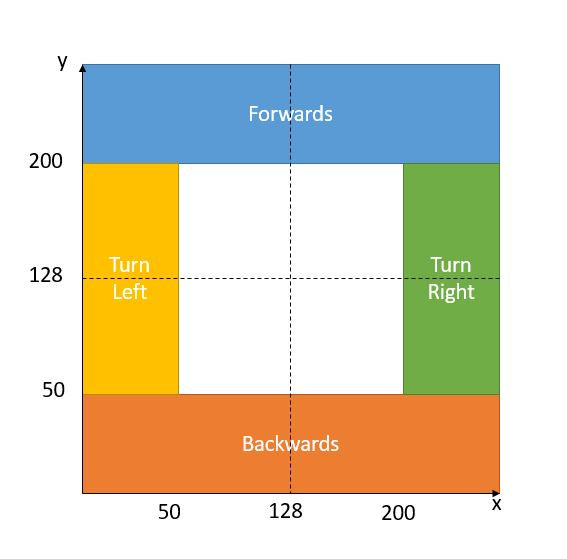
\includegraphics[scale=0.8]{Manual_mode_movement.jpg}
		\centering
		\caption{Movement from Joystick}
	\end{figure}
	
	
	\subsubsection{Manual Mode Flowchart}
	
	\begin{figure}[h]
		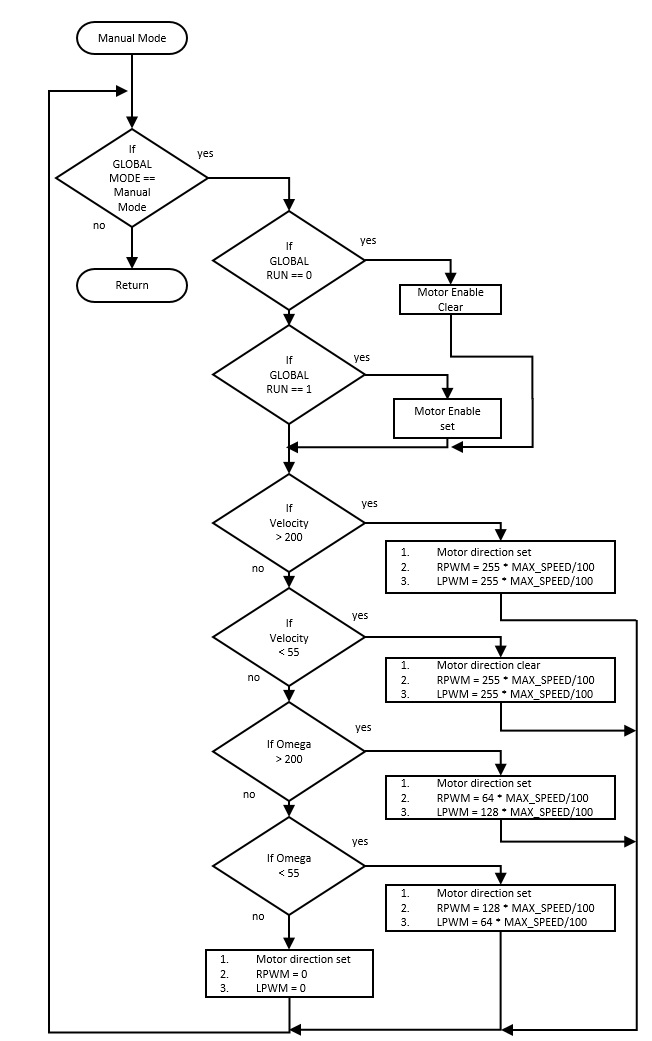
\includegraphics[scale=0.8]{Manual_mode_flow.jpg}
		\centering
		\caption{Manual Mode Flowchart}
	\end{figure}
	
	
\end{document}